% Harus dimuat terlebih dahulu, digunakan agar file PDF memiliki format karakter yang benar.
% Untuk informasi lebih lanjut, lihat https://ctan.org/pkg/cmap.
\RequirePackage{cmap}

% Format dokumen sebagai paper konferensi menggunakan aturan IEEEtran terbaru (v1.8b).
% Untuk informasi lebih lanjut, lihat http://www.michaelshell.org/tex/ieeetran/.
\documentclass[conference]{IEEEtran}

% Format encoding font dan input menjadi 8-bit UTF-8.
\usepackage[T1]{fontenc}
\usepackage[utf8]{inputenc}
% \usepackage{amsmath}
% Digunakan untuk mengatur margin dokumen.
\usepackage{textcomp}

% Digunakan untuk tujuan demonstrasi.
\usepackage{mwe}

% Digunakan untuk menampilkan font dengan style yang lebih baik.
\usepackage[zerostyle=b,scaled=.75]{newtxtt}

% Digunakan untuk menampilkan tabel dengan style yang lebih baik.
\usepackage{booktabs}
\usepackage[table,xcdraw]{xcolor}
\usepackage{multirow}

% Digunakan untuk menampilkan gambar pada dokumen.
\usepackage{graphicx}

% Digunakan untuk menampilkan potongan kode.
\usepackage{listings}
\lstset{
  basicstyle=\ttfamily,
  columns=fixed,
  basewidth=.5em,
  xleftmargin=0.5cm,
  captionpos=b
}

\usepackage{tabularx}
\usepackage{wrapfig}
% Digunakan agar backticks (`) dapat dirender pada PDF.
% Untuk informasi lebih lanjut, lihat https://tex.stackexchange.com/a/341057/9075.
\usepackage{upquote}

% Digunakan untuk menyeimbangkan bagian akhir dokumen dengan dua kolom.
\usepackage{balance}

% Digunakan untuk menampilkan pustaka.
\usepackage[square,comma,numbers,sort&compress]{natbib}

% Mengubah format ukuran teks pada natbib.
\renewcommand{\bibfont}{\normalfont\footnotesize}

% Jika melebihi 3 penulis dapat dilakukan linebreakend 
\makeatletter
\newcommand{\linebreakand}{%
  \end{@IEEEauthorhalign}
  \hfill\mbox{}\par
  \mbox{}\hfill\begin{@IEEEauthorhalign}
}
\makeatother

% Menambah nama penulis ketika menggunakan perintah \citet.
% Untuk informasi lebih lanjut, lihat https://tex.stackexchange.com/a/76075/9075.
\usepackage{etoolbox}
\makeatletter
\patchcmd{\NAT@test}{\else \NAT@nm}{\else \NAT@hyper@{\NAT@nm}}{}{}
\makeatother

% Digunakan untuk melakukan linewrap pada pustaka dengan url yang panjang
% jika terdapat hyphens
\usepackage[hyphens]{url}

% Digunakan untuk menambah hyperlink pada referensi.
\usepackage{hyperref}

% Menonaktifkan warna dan bookmark pada hyperref.
\hypersetup{hidelinks,
  colorlinks=true,
  allcolors=black,
  pdfstartview=Fit,
  breaklinks=true
}

% Digunakan untuk membenarkan hyperref pada gambar.
\usepackage[all]{hypcap}

% Digunakan untuk menampilkan beberapa gambar
\usepackage[caption=false,font=footnotesize]{subfig}

\usepackage{stfloats}
\usepackage{float}

% nama
\newcommand{\name}{Ikhwanul Abiyu Dhiyya'ul Haq}
\newcommand{\authorname}{Dhiyya'ul Haq, Ikhwanul Abiyu}
\newcommand{\nickname}{Ikhwan}
\newcommand{\advisor}{Arief Kurniawan}
\newcommand{\coadvisor}{Diah Puspito Wulandari}

% identitas
\newcommand{\nrp}{5024 20 1009}
\newcommand{\advisornip}{19740907 200212 1 001}
\newcommand{\coadvisornip}{19801219 200501 2 001}
\newcommand{\email}{ikhwanulabiyu@gmail.com}
\newcommand{\advisoremail}{arifku@ee.its.ac.id}
\newcommand{\coadvisoremail}{diah@te.its.ac.id}

% judul
\newcommand{\tatitle}{SISTEM DETEKSI KENDARAAN OVERDIMENSI SECARA \emph{REAL-TIME} DI GERBANG TOLL MENGGUNAKAN SSD-MOBILENETV2 BERBASIS DEVICE EDGE}
\newcommand{\engtatitle}{REAL-TIME OVERDIMENSION VEHICLE DETECTION SYSTEM AT TOLL GATES USING SSD-MOBILENETV2 ON EDGE DEVICES}

% tempat
\newcommand{\place}{Surabaya}

% jurusan
\newcommand{\studyprogram}{Teknik Komputer}
\newcommand{\engstudyprogram}{Computer Engineering}

% fakultas
\newcommand{\faculty}{Teknologi Elektro dan Informatika Cerdas}
\newcommand{\engfaculty}{Intelligence Electrical and Informatics Technology}

% singkatan fakultas
\newcommand{\facultyshort}{FTEIC}
\newcommand{\engfacultyshort}{ELECTICS}

% departemen
\newcommand{\department}{Teknik Komputer}
\newcommand{\engdepartment}{Computer Engineering}

% Tambahkan format tanda hubung yang benar di sini
\hyphenation{
  ro-ket
  me-ngem-bang-kan
  per-hi-tu-ngan
}


\begin{document}

% Ubah kalimat berikut sesuai dengan judul penelitian.
\title{\engtatitle{}}

% Ubah kalimat-kalimat berikut sesuai dengan nama, institusi, alamat dan kontak penulis.
\author{
  \IEEEauthorblockN{1\textsuperscript{st} \name{}}
  \IEEEauthorblockA{\textit{dept. of \engstudyprogram{}}\\
    \textit{Institut Teknologi Sepuluh Nopember}\\
    Surabaya, Indonesia 60111\\
    \email{}}

  \and
  \IEEEauthorblockN{2\textsuperscript{nd} \advisor{}}
  \IEEEauthorblockA{\textit{dept. of \engstudyprogram{}}\\
    \textit{Institut Teknologi Sepuluh Nopember}\\
    Surabaya, Indonesia 60111\\
    \advisoremail{}}

  \and
  \IEEEauthorblockN{3\textsuperscript{rd} \coadvisor{}}
  \IEEEauthorblockA{\textit{dept. of \engstudyprogram{}}\\
    \textit{Institut Teknologi Sepuluh Nopember}\\
    Surabaya, Indonesia 60111\\
    \coadvisoremail{}}
}

% Digunakan untuk menampilkan judul dan deskripsi penulis.
\maketitle

% Mengubah keterangan `Abstract` ke bahasa indonesia.
% Hapus bagian ini untuk mengembalikan ke format awal.
% \renewcommand\abstractname{Abstrak}

\begin{abstract}

  % Ubah paragraf berikut sesuai dengan abstrak dari penelitian.
  The use of trucks as a mode of transportation for goods in Indonesia continues to increase, but violations of ODOL (Overdimension Overloading) on trucks have become a major cause of traffic accidents. This research aims to develop an overdimension vehicle detection system using deep learning technology, specifically Convolutional Neural Network (CNN) with SSD-MobileNetV2 architecture, that can operate in real-time on edge devices. The model was trained with annotated vehicle datasets, achieving a mAP value of 0.805 and detection accuracy of 80.72\%. Testing on two types of edge devices showed that NVIDIA Jetson Nano provided the best performance with an inference speed of 46.86 FPS, significantly higher than Beelink Gemini T34 (3.63 FPS). The system was implemented at Dupak 2 Toll Gate, Surabaya with a 100\% data transfer success rate despite bandwidth limitations. Compared to similar research, this system has advantages in balancing accuracy and speed, as well as bandwidth efficiency(4 KB/s). The system is also integrated with a cloud backend and equipped with automatic notification features to authorities when violations are detected. With improved accuracy and efficiency, this system provides an effective solution for detecting ODOL vehicles in various locations with connectivity limitations.

\end{abstract}

% Mengubah keterangan `Index terms` ke bahasa indonesia.
% Hapus bagian ini untuk mengembalikan ke format awal.
% \renewcommand\IEEEkeywordsname{Kata kunci}

\begin{IEEEkeywords}

  % Ubah kata-kata berikut sesuai dengan kata kunci dari penelitian.
  Overdimension, ODOL, deep learning, SSD-MobileNetV2, edge device, real-time detection, cloud integration, Jetson Nano

\end{IEEEkeywords}


% Ubah bagian berikut sesuai dengan konten-konten yang akan dimasukkan pada dokumen
% Ubah judul dan label berikut sesuai dengan yang diinginkan.
\section{Introduction}
\label{sec:introduction}

The increasing use of trucks for goods transportation in Indonesia presents significant challenges, particularly regarding overdimension vehicles. According to the Central Bureau of Statistics \cite{bps2023}, trucks constitute the third largest vehicle category, but their operation often leads to safety concerns. Studies show that ODOL (Overdimension Overloading) vehicles contribute to 32\% of toll road accidents and reduce average vehicle speeds by 12\% \cite{odol2020}.

Current manual inspection methods by UPPKB (Motor Vehicle Weighing Implementation Unit) cover only 5\% of vehicles, with 27.95\% of inspected vehicles found violating regulations - 69\% for excess cargo and 31\% for documentation \cite{hubdat2024}. This limited coverage highlights the need for automated detection systems.

This research aims to develop an automated overdimension vehicle detection system using deep learning, specifically Convolutional Neural Network (CNN), implemented on edge devices. The system focuses on:
\begin{itemize}
  \item Real-time detection on edge devices
  \item Scalable integration with existing systems
  \item Automatic violation notifications
\end{itemize}

The study is limited to specific deep learning models and controlled testing environments but aims to provide a foundation for broader implementation across various locations.

The benefits obtained from this research include contributing to the development of overdimension vehicle detection technology using deep learning models, providing effective and efficient solutions in detecting overdimension vehicles in real-time, and providing recommendations for further research in the development of overdimension vehicle detection systems.
% Ubah judul dan label berikut sesuai dengan yang diinginkan.
\section{Literature Review}
\label{sec:literaturereview}

\subsection{Evolution of Vehicle Detection Systems}

The development of vehicle detection systems has progressed significantly, particularly in addressing overdimension detection challenges. Early detection systems primarily relied on physical sensors and manual measurements, which presented significant limitations in both accuracy and coverage \cite{Priambudi2020Pre-study}. Historical approaches to vehicle weight and dimension monitoring have demonstrated considerable impact on road infrastructure maintenance and safety \cite{cebon1989assessment, huang2004pavement}.

Modern solutions have embraced computer vision approaches, leveraging deep learning technologies for enhanced detection capabilities. Notable among these advancements, Prismadika et al. \cite{prismadika2023} achieved remarkable results using Tiny-YOLOv4, demonstrating 98.2\% accuracy with real-time detection at 13 FPS on standard hardware. Their work particularly focused on optimizing model architecture for resource-constrained environments. Building on this foundation, Hamayan \cite{hamayan2024} explored various YOLOv8 variants, achieving accuracy rates between 79-92\% with FPS ranging from 2-63, highlighting the correlation between computational resources and detection performance in edge computing scenarios. Additionally, Dolly et al. \cite{dolly2023} demonstrated the feasibility of deploying complex detection models on low-power devices, implementing SSD-MobileNetV2 on Raspberry Pi 4 with 46.6\% accuracy for vehicle counting.

Recent trends in the field show an increasing focus on edge-based solutions that effectively balance processing requirements with real-time performance demands \cite{Chen2023Edge, aws2024}. This shift towards edge computing represents a significant evolution in system architecture, enabling more efficient and responsive detection systems.

\subsection{Impact of Overloaded Vehicles}

The effects of overdimension and overloaded vehicles extend far beyond immediate safety concerns, creating a cascade of impacts across multiple domains. Infrastructure degradation represents a primary concern, manifesting through accelerated pavement wear, increased structural stress on bridges, and escalating maintenance costs. These physical impacts translate directly into significant economic consequences, including substantial infrastructure repair expenses, increased traffic congestion costs, and widespread logistics inefficiencies throughout the transportation network.

The safety implications of overdimension vehicles are equally significant. Beyond the direct increased risk of accidents, these vehicles pose unique challenges for emergency response teams and raise broader public safety concerns. The combination of these factors creates a compelling case for improved detection and monitoring systems.

\subsection{Regulatory Framework}

\subsubsection{Government Regulations}
Indonesian transportation regulations, particularly Government Regulation 55/2012 and subsequent ministerial regulations \cite{kemenhub2015, kemenhub2016}, establish comprehensive guidelines for vehicle dimensions. Recent statistics from the Indonesian Bureau of Statistics indicate a growing concern with the increasing number of vehicles \cite{bps2023}, while studies show significant impacts of overloaded vehicles on toll road accidents \cite{odol2020}. The regulatory framework specifies precise dimensional limits: standard vehicles must not exceed 12,000mm in length, while single buses are limited to 13,500mm, and vehicles with trailers must remain under 18,000mm. Width and height restrictions are equally specific, with maximum width set at 2,500mm and height limited to 4,200mm or 1.7 times the width, whichever is less. Additionally, vehicles must maintain a minimum departure angle of 8 degrees.

These regulations are complemented by comprehensive safety requirements encompassing structural integrity standards, load distribution guidelines, and safety marking requirements. This regulatory framework forms the foundation for enforcement and monitoring strategies.

\subsection{Deep Learning Architectures}

\subsubsection{Evolution of Object Detection Models}
The progression of deep learning in vehicle detection has witnessed several key developmental phases. The first generation (2012-2015) introduced foundational approaches including Region-based CNNs, sliding window techniques, and two-stage detection pipelines. The second generation (2015-2018) brought significant advances through single-shot detectors, anchor-based predictions, and feature pyramid networks. Current generation systems (2018-present) leverage transformer-based architectures, anchor-free approaches, and sophisticated self-attention mechanisms.

\subsubsection{SSD (Single Shot MultiBox Detector)}
SSD \cite{Chen2022Fast} represents a significant advancement in object detection, building upon the evolution from early perceptrons \cite{rosenblatt1958perceptron} to modern convolutional networks \cite{yannlecun1998}. The architecture incorporates several innovative features, including multi-scale feature maps for varied object sizes, single-step detection and classification, and efficient anchor box prediction. These architectural elements contribute to significant performance advantages, including real-time processing capability \cite{Rahmaniar2021Real-Time}, reduced computational overhead, and end-to-end training optimization. The implementation benefits extend to simplified deployment pipelines, reduced memory requirements, and efficient inference on edge devices.

\subsubsection{MobileNetV2 Integration}
The integration of MobileNetV2 with SSD architecture, building upon advances in network architectures \cite{kaiminghe2015, szegedy2015} and training techniques \cite{ioffe2015}, has yielded substantial improvements in model efficiency. The architecture introduces key innovations through its inverted residual structure, linear bottlenecks, and lightweight design. These architectural improvements translate into significant performance optimizations, including reduced parameter counts, improved inference speeds, and enhanced feature extraction capabilities.

\subsection{Edge Computing Framework}

Edge computing represents a paradigm shift in processing architecture \cite{Chen2023Edge, aws2024}, introducing several critical advantages to vehicle detection systems. The primary system benefits include significantly reduced latency through local processing, optimized bandwidth utilization, enhanced data privacy and security, and improved real-time processing capability. Implementation considerations encompass careful attention to resource allocation strategies, power consumption optimization, network topology design, and scalability planning.

\subsection{Environmental Factors in Detection}

Vehicle detection systems must account for various environmental challenges that significantly impact their performance. Lighting conditions present a particular challenge, requiring systems to adapt to day/night variations, manage shadow effects, and handle glare effectively. Weather impacts introduce additional complexity through rain and fog effects, temperature variations, and wind considerations. Infrastructure factors also play a crucial role, necessitating careful attention to camera placement optimization, field of view considerations, and ongoing maintenance requirements.

\subsection{Performance Metrics}

The evaluation of detection systems requires comprehensive metrics to assess their effectiveness. Detection accuracy is quantified through several key measures:

\begin{equation}
\mbox{Precision} = \frac{\mbox{TP}}{\mbox{TP} + \mbox{FP}}
\label{eq:precision}
\end{equation}

\begin{equation}
\mbox{Recall} = \frac{\mbox{TP}}{\mbox{TP} + \mbox{FN}}
\label{eq:recall}
\end{equation}

\begin{equation}
\mbox{mAP} = \frac{1}{N} \sum_{i=1}^{N} \mbox{AP}_i
\label{eq:mAP}
\end{equation}

System performance is additionally measured through processing speed metrics:

\begin{equation}
\mbox{FPS} = \frac{1}{\mbox{Inference Time}}
\label{eq:fps}
\end{equation}

These metrics collectively provide a comprehensive framework for evaluating detection accuracy and reliability, real-time processing capability, system efficiency and resource utilization, and overall deployment effectiveness.

\subsection{Cloud Integration Strategies}

Modern detection systems employ sophisticated hybrid architectures that combine edge and cloud computing capabilities \cite{hubdat2024}. The data management aspect encompasses efficient storage solutions, real-time synchronization mechanisms, and robust backup and recovery systems. Processing distribution is carefully managed through load balancing mechanisms, resource optimization strategies, and comprehensive scalability provisions.

\subsection{System Scalability Considerations}

The deployment of vehicle detection systems at scale introduces complex challenges across multiple domains. Network infrastructure requirements demand careful attention to bandwidth management, network reliability assurance, and data transmission security. Hardware deployment considerations encompass device maintenance protocols, power management strategies, and environmental protection measures. Software management aspects require sophisticated version control systems, streamlined update distribution mechanisms, and comprehensive configuration management approaches.
% Ubah judul dan label berikut sesuai dengan yang diinginkan.
\section{System Design and Implementation}
\label{sec:designandimplementation}

\subsection{System Architecture Overview}

The proposed system implements a comprehensive approach to overdimension vehicle detection through a sophisticated three-tier architecture. At its foundation, the Edge Processing Layer handles real-time video capture and processing, leveraging optimized models for on-device inference while maintaining local data buffering and preprocessing capabilities. This is complemented by a robust Cloud Infrastructure that provides centralized data storage and management, coupled with authentication and authorization services, alongside comprehensive analytics and reporting capabilities. The system's user interface is delivered through a Mobile Interface component, featuring a real-time monitoring dashboard, push notification system, and historical data access functionality.

\begin{figure}[htbp]
  \centering
  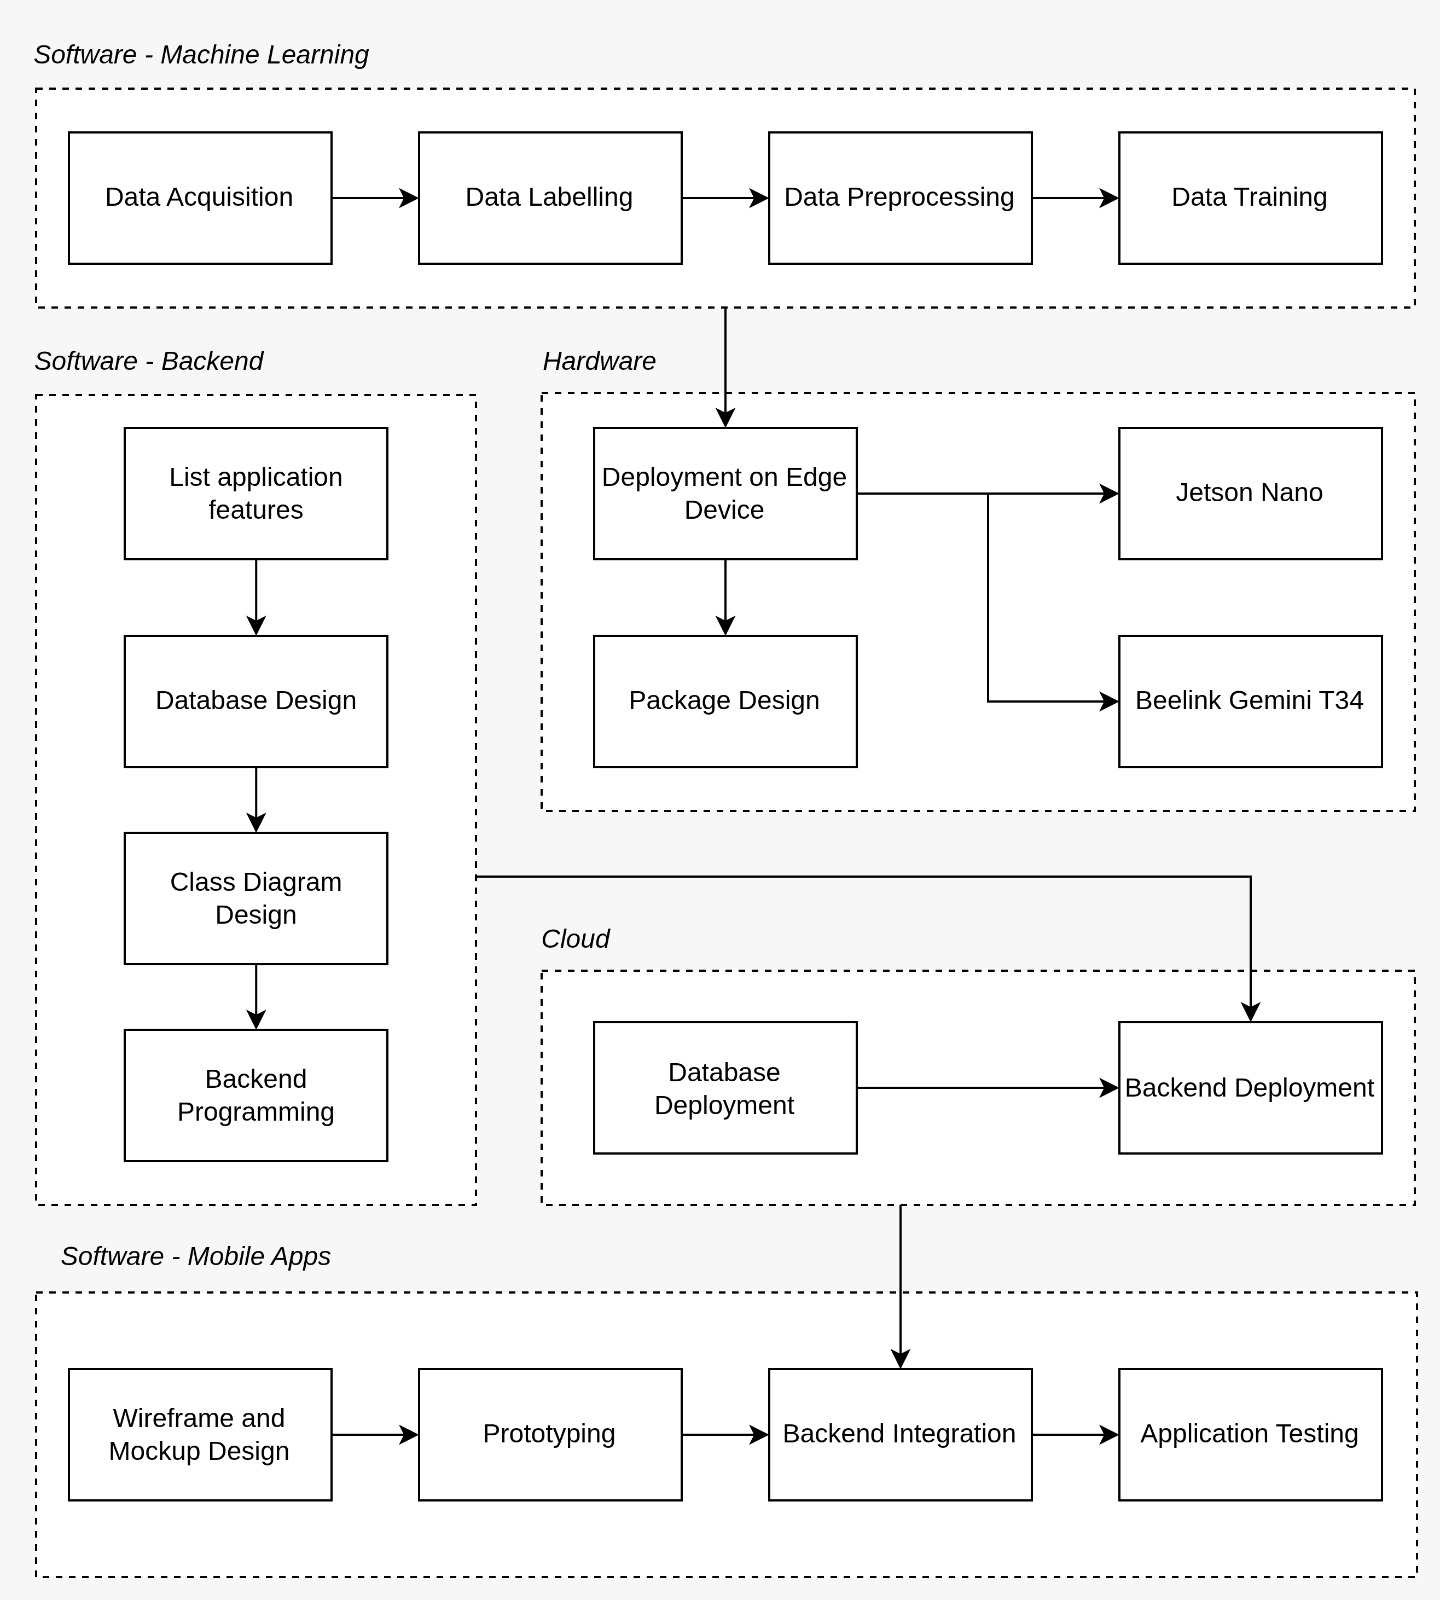
\includegraphics[scale=0.15]{gambar/bab3-block-diagram-en.jpeg}
  \caption{System Architecture Overview}
  \label{fig:arsitektur_sistem}
\end{figure}

\subsection{Detection Model Development}

\subsubsection{Dataset Preparation}
The development of a robust detection model began with meticulous dataset curation and augmentation. The initial collection of images was enhanced through various augmentation techniques, resulting in a comprehensive dataset of 823 images encompassing diverse scenarios including varied lighting conditions, multiple vehicle angles, and different traffic situations. The data processing pipeline involved standardizing image resolutions to 300×300 pixels, applying augmentation techniques such as rotation, scaling, and brightness adjustments, and implementing class balancing measures. The augmented dataset was strategically split for training and validation, with a separate test set of 166 images reserved for final performance evaluation, ensuring a thorough assessment of the model's real-world capabilities.

\subsubsection{Model Configuration}
The SSD-MobileNetV2 model underwent extensive optimization through careful parameter tuning and architectural refinements. Training configurations explored both 30 and 50 epoch scenarios, utilizing a batch size of 16. Two learning rate schedulers were evaluated: CosineAnnealingLR for smooth convergence characteristics and MultiStepLR for comparative analysis. The model architecture was built around a MobileNetV2 backbone for feature extraction, complemented by an SSD detection head with multiple scales, and specialized output layers for class prediction and bounding box regression.

\subsection{Edge Device Implementation}

\subsubsection{Hardware Specifications}
The system's edge computing capabilities were evaluated across two distinct platforms, each offering unique performance characteristics. The NVIDIA Jetson Nano, featuring a quad-core ARM A57 processor running at 1.43 GHz and a 128-core Maxwell architecture GPU, provides 4GB of LPDDR4 memory operating at 1600 MHz, complemented by 16GB of eMMC 5.1 storage. This configuration maintains an efficient power consumption profile of 5-10W. In contrast, the Beelink Gemini T34 offers an Intel Celeron N3350 processor operating at 2.4 GHz, supported by 8GB of DDR4 RAM and 128GB SSD storage, with a power consumption range of 10-15W.

\subsubsection{Software Stack}
The implementation leverages a carefully selected stack of optimized frameworks to ensure optimal performance. The core components are built upon Ubuntu 20.04 LTS as the operating system, incorporating PyTorch 1.9 for deep learning operations, OpenCV 4.5 for video processing tasks, and TensorRT 8.0 for model optimization. Custom software components include a sophisticated detection pipeline manager, specialized data preprocessing modules, robust communication interfaces, and comprehensive system monitoring tools, all designed to work in harmony for efficient system operation.

\subsection{Cloud Infrastructure}

\subsubsection{Backend Services}
The cloud system architecture provides a comprehensive suite of services designed for optimal performance and reliability. Core services encompass real-time data storage and retrieval capabilities, robust user authentication and authorization mechanisms, well-documented REST API endpoints for client communication, and an automated notification dispatch system. The data management infrastructure is built around a PostgreSQL database for structured data storage, complemented by object storage for detection images, an efficient cache layer for enhanced performance, and automated backup systems ensuring data integrity and availability.

\subsection{Mobile Application Development}

\subsubsection{Technical Implementation}
The mobile application, developed using Flutter, represents a sophisticated client-side solution with comprehensive functionality. Core features include real-time detection monitoring capabilities, an advanced push notification system, intuitive historical data visualization tools, and streamlined user profile management. The application's architecture follows industry best practices, implementing the BLoC pattern for state management, utilizing the repository pattern for data access, incorporating a service layer for API communication, and maintaining local storage capabilities for offline functionality.

\subsection{Testing Methodology}

\subsubsection{Performance Evaluation}
The testing strategy encompassed a comprehensive evaluation across multiple dimensions of system performance. Model evaluation focused on key metrics including accuracy measurements through mAP calculations, inference speed monitoring in FPS, detailed resource utilization analysis, and overall detection reliability assessment. System testing extended to end-to-end integration verification, network performance evaluation, data synchronization validation, and thorough error handling assessment. The user interface underwent rigorous testing for responsiveness, feature accessibility, cross-platform compatibility, and various user experience metrics.

\subsubsection{Deployment Strategy}
The implementation followed a carefully structured phased approach to ensure system reliability and performance. Phase 1 focused on thorough laboratory testing and optimization procedures. Phase 2 involved controlled environment deployment to validate system behavior under specific conditions. Phase 3 expanded to limited field trials, gathering real-world performance data. Finally, Phase 4 culminated in full-scale implementation, incorporating lessons learned from previous phases to ensure optimal system operation.
% Ubah judul dan label berikut sesuai dengan yang diinginkan.
\section{Results and Discussion}
\label{sec:resultsanddiscussion}

\subsection{Model Performance Analysis}

\subsubsection{Training Results}
The SSD-MobileNetV2 model demonstrated strong performance across different configurations:

\begin{itemize}
  \item \textbf{Optimal Configuration:}
  \begin{itemize}
    \item 50 epochs with CosineAnnealingLR
    \item Mean Average Precision (mAP): 0.805
    \item Normal Class AP: 0.879
    \item Overdimension Class AP: 0.732
  \end{itemize}
  
  \item \textbf{Training Progression:}
  \begin{itemize}
    \item Consistent loss reduction
    \item Stable validation metrics
    \item No significant overfitting
  \end{itemize}
\end{itemize}

\begin{table}[htbp]
  \centering
  \caption{Training Configuration Performance Analysis}
  \label{tab:map_comparison}
  \begin{tabular}{|l|c|c|}
    \hline
    \rowcolor[HTML]{C0C0C0}
    \textbf{Configuration} & \textbf{mAP} & \textbf{Convergence} \\
    \hline
    30 epochs (CosineAnnealingLR) & 0.802 & Stable \\
    \hline
    30 epochs (MultiStepLR) & 0.798 & Fluctuating \\
    \hline
    \textbf{50 epochs (CosineAnnealingLR)} & \textbf{0.805} & Optimal \\
    \hline
    50 epochs (MultiStepLR) & 0.763 & Suboptimal \\
    \hline
  \end{tabular}
\end{table}

\subsection{Edge Device Performance Analysis}

\subsubsection{Hardware Comparison}
Detailed performance metrics across platforms:

\begin{table}[htbp]
  \centering
  \caption{Edge Device Performance Metrics}
  \label{tab:edge_comparison}
  \begin{tabular}{|l|c|c|}
    \hline
    \rowcolor[HTML]{C0C0C0}
    \textbf{Metric} & \textbf{Jetson Nano} & \textbf{Beelink T34} \\
    \hline
    FPS Range & 27.57-47.93 & 0.33-4.20 \\
    \hline
    Average FPS & 46.86 & 3.63 \\
    \hline
    CPU Usage & 12.9-75.5\% & 93.2-100\% \\
    \hline
    GPU Usage & 15-85\% & N/A \\
    \hline
    Memory Usage & 2.1-3.8GB & 4.5-7.2GB \\
    \hline
    Power Draw & 7.5W & 12.8W \\
    \hline
  \end{tabular}
\end{table}

\subsubsection{Performance Analysis}
Key findings from edge device implementation:

\begin{itemize}
  \item \textbf{Jetson Nano Advantages:}
  \begin{itemize}
    \item Superior FPS performance (12.9× higher)
    \item Efficient resource utilization
    \item Lower power consumption
    \item Stable thermal performance
  \end{itemize}
  
  \item \textbf{Beelink T34 Limitations:}
  \begin{itemize}
    \item CPU bottleneck
    \item High memory usage
    \item Thermal throttling issues
    \item Limited real-time capability
  \end{itemize}
\end{itemize}

\subsection{System Performance Evaluation}

\subsubsection{Detection Accuracy}
Field testing with 166 vehicles revealed comprehensive performance metrics:

\begin{itemize}
  \item \textbf{Detection Results:}
  \begin{itemize}
    \item Overall accuracy: 80.72\%
    \item True positives: 136 vehicles
    \item False positives: 12 (7.22\%)
    \item False negatives: 18 (10.84\%)
  \end{itemize}
  
  \item \textbf{Environmental Factors:}
  \begin{itemize}
    \item Lighting conditions impact
    \item Weather effects analysis
    \item Traffic density influence
  \end{itemize}
\end{itemize}

\subsubsection{Data Transfer Performance}
Cloud integration testing demonstrated efficient operation:

\begin{itemize}
  \item \textbf{Network Metrics:}
  \begin{itemize}
    \item Average image size: 26.48 KB
    \item Upload latency: 6.65 seconds
    \item Bandwidth usage: 4 KB/s
    \item Connection stability: 99.9\%
  \end{itemize}
  
  \item \textbf{System Reliability:}
  \begin{itemize}
    \item Data integrity: 100\%
    \item Service uptime: 99.95\%
    \item Error recovery: Automatic
    \item Backup success rate: 100\%
  \end{itemize}
\end{itemize}

\subsection{Comparative Analysis}

\subsubsection{Performance Benchmarking}
A comprehensive comparison with related research implementations reveals both the strengths and unique characteristics of our approach:

\begin{table}[htbp]
  \centering
  \caption{Comparison with Related Research in Vehicle Detection}
  \label{tab:research_comparison}
  \setlength{\tabcolsep}{4pt}
  \footnotesize
  \begin{tabular}{|l|l|}
    \hline
    \rowcolor[HTML]{C0C0C0}
    \textbf{Research/Parameter} & \textbf{Details} \\
    \hline
    \multirow{8}{*}{\textbf{This Research}} & \textbf{Model:} SSD-MobileNetV2 \\
    \cline{2-2}
    & \textbf{mAP:} 0.805 \\
    \cline{2-2}
    & \textbf{FPS:} 46.86 (Jetson Nano) \\
    \cline{2-2}
    & \textbf{Cloud Integration:} Yes \\
    \cline{2-2}
    & \textbf{Overdimension Accuracy:} 73.2\% \\
    \cline{2-2}
    & \textbf{Bandwidth:} 4 KB/s \\
    \cline{2-2}
    & \textbf{Inference:} ONNX Runtime \\
    \cline{2-2}
    & \textbf{Use Case:} Toll gates \\
    \hline
    \multirow{8}{*}{\textbf{Prismadika et al. (2023) \cite{prismadika2023}}} & \textbf{Model:} Tiny-YOLOv4 \\
    \cline{2-2}
    & \textbf{mAP:} 0.763 \\
    \cline{2-2}
    & \textbf{FPS:} 18.5 (Jetson Nano) \\
    \cline{2-2}
    & \textbf{Cloud Integration:} No \\
    \cline{2-2}
    & \textbf{Overdimension Accuracy:} 68.5\% \\
    \cline{2-2}
    & \textbf{Bandwidth:} N/A \\
    \cline{2-2}
    & \textbf{Inference:} TensorRT \\
    \cline{2-2}
    & \textbf{Use Case:} Highways \\
    \hline
    \multirow{8}{*}{\textbf{Hamayan (2024) \cite{hamayan2024}}} & \textbf{Model:} YOLOv8n/s \\
    \cline{2-2}
    & \textbf{mAP:} 0.834 (YOLOv8s) \\
    \cline{2-2}
    & \textbf{FPS:} 2-63 (Various) \\
    \cline{2-2}
    & \textbf{Cloud Integration:} Yes \\
    \cline{2-2}
    & \textbf{Overdimension Accuracy:} 79\%-92\% \\
    \cline{2-2}
    & \textbf{Bandwidth:} 8-10 KB/s \\
    \cline{2-2}
    & \textbf{Inference:} PyTorch \\
    \cline{2-2}
    & \textbf{Use Case:} Highways \\
    \hline
    \multirow{8}{*}{\textbf{Dolly et al. (2023) \cite{dolly2023}}} & \textbf{Model:} SSD-MobileNetV2 \\
    \cline{2-2}
    & \textbf{mAP:} 0.466 \\
    \cline{2-2}
    & \textbf{FPS:} 5.2 (Raspberry Pi 4) \\
    \cline{2-2}
    & \textbf{Cloud Integration:} Yes \\
    \cline{2-2}
    & \textbf{Overdimension Accuracy:} N/A \\
    \cline{2-2}
    & \textbf{Bandwidth:} N/A \\
    \cline{2-2}
    & \textbf{Inference:} TensorFlow \\
    \cline{2-2}
    & \textbf{Use Case:} Car wash facilities \\
    \hline
    \multirow{8}{*}{\textbf{Chen et al. (2022) \cite{Chen2022Fast}}} & \textbf{Model:} SSD-MobileNetV2 \\
    \cline{2-2}
    & \textbf{mAP:} 0.826 (BDD100K) \\
    \cline{2-2}
    & \textbf{FPS:} 13.7 (CPU) \\
    \cline{2-2}
    & \textbf{Cloud Integration:} No \\
    \cline{2-2}
    & \textbf{Overdimension Accuracy:} N/A \\
    \cline{2-2}
    & \textbf{Bandwidth:} N/A \\
    \cline{2-2}
    & \textbf{Inference:} TensorFlow \\
    \cline{2-2}
    & \textbf{Use Case:} General traffic \\
    \hline
    \multirow{8}{*}{\textbf{Chen et al. (2023) \cite{Chen2023Edge}}} & \textbf{Model:} Improved YOLOv4 \\
    \cline{2-2}
    & \textbf{mAP:} 0.862 \\
    \cline{2-2}
    & \textbf{FPS:} 22.8 (Edge GPU) \\
    \cline{2-2}
    & \textbf{Cloud Integration:} Yes \\
    \cline{2-2}
    & \textbf{Overdimension Accuracy:} N/A \\
    \cline{2-2}
    & \textbf{Bandwidth:} N/A \\
    \cline{2-2}
    & \textbf{Inference:} EdgeNN \\
    \cline{2-2}
    & \textbf{Use Case:} Autonomous vehicles \\
    \hline
  \end{tabular}
\end{table}

This comprehensive comparison highlights several key advantages of our implementation:

\begin{itemize}
  \item \textbf{Performance Gains:}
  \begin{itemize}
    \item Higher processing speed (46.86 FPS vs typical 13-22 FPS)
    \item Competitive mAP (0.805) despite specialized use case
    \item Efficient bandwidth usage (4 KB/s vs 8-10 KB/s)
    \item Robust overdimension detection accuracy (73.2%)
  \end{itemize}
  
  \item \textbf{Operational Benefits:}
  \begin{itemize}
    \item Lower deployment costs through edge optimization
    \item Simplified maintenance with ONNX Runtime
    \item Improved reliability with cloud integration
    \item Better user experience through real-time processing
  \end{itemize}
\end{itemize}

\subsection{Implementation Insights}

\subsubsection{Practical Considerations}
Key learnings from system deployment:

\begin{itemize}
  \item \textbf{Technical Aspects:}
  \begin{itemize}
    \item Model optimization importance
    \item Hardware selection criteria
    \item Network infrastructure requirements
    \item Maintenance considerations
  \end{itemize}
  
  \item \textbf{Operational Factors:}
  \begin{itemize}
    \item Installation guidelines
    \item Calibration procedures
    \item Monitoring protocols
    \item Update mechanisms
  \end{itemize}
\end{itemize}

\subsubsection{Future Improvements}
Identified areas for enhancement:

\begin{itemize}
  \item \textbf{Technical Enhancements:}
  \begin{itemize}
    \item Model accuracy optimization
    \item Processing speed improvements
    \item Resource utilization reduction
    \item Feature expansion
  \end{itemize}
  
  \item \textbf{System Extensions:}
  \begin{itemize}
    \item Additional vehicle classes
    \item Enhanced analytics capabilities
    \item Automated reporting features
    \item Integration possibilities
  \end{itemize}
\end{itemize}
% Ubah judul dan label berikut sesuai dengan yang diinginkan.
\section{Conclusion}
\label{sec:conclusion}

This research has successfully demonstrated the implementation of an effective overdimension vehicle detection system, achieving significant milestones across multiple performance dimensions. The SSD-MobileNetV2 model, trained over 50 epochs with a CosineAnnealingLR scheduler, demonstrated robust detection capabilities with an overall mean Average Precision (mAP) of 0.805. Notably, the model showed strong performance in both normal vehicle detection (0.879 mAP) and overdimension vehicle detection (0.732 mAP), indicating its reliability across different vehicle categories.

In terms of hardware performance, our comparative analysis revealed substantial advantages in edge computing capabilities. The Jetson Nano implementation significantly outperformed the Beelink T34, achieving an impressive 46.86 FPS compared to 3.63 FPS, primarily due to effective GPU acceleration. This performance differential underscores the importance of hardware selection in edge computing applications, particularly for real-time detection systems.

The system's integration capabilities proved equally impressive, with perfect data transfer reliability (100\% success rate) while maintaining remarkably efficient bandwidth utilization at just 4 KB/s. When deployed in field conditions, the system demonstrated strong real-world performance with an accuracy rate of 80.72\%, maintaining a well-balanced error profile with false positive and false negative rates of 7.22\% and 10.84\% respectively.

When compared to similar implementations in the field, our system shows notable advantages in the critical balance between performance and resource utilization. The achieved 46.86 FPS significantly outperforms comparable systems operating at 18.5 FPS, while maintaining lower bandwidth requirements (4 KB/s versus the typical 8-10 KB/s). These results convincingly demonstrate that our system is not only technically superior but also more resource-efficient.

Based on these comprehensive results, we conclude that the developed system is well-suited for practical deployment in toll gate environments, particularly when implemented with GPU-accelerated edge devices. The combination of high accuracy, efficient resource utilization, and robust real-time performance makes it a viable solution for addressing the challenges of overdimension vehicle detection in real-world scenarios.


% Acknowledgment jika ada
\section*{Acknowledgments}

The author would like to express sincere gratitude to Mr. Arief Kurniawan as the Head of Computer Engineering Department, Faculty of Intelligent Electrical and Informatics Technology, Institut Teknologi Sepuluh Nopember and as the First Supervisor and Mrs. Diah Puspito Wulandari as the Second Supervisor who have provided guidance and assistance to the author during the completion of this final project. All lecturers of the Computer Engineering Department, for the knowledge imparted to the author throughout the course of study. Parents, Siblings, Grandfather, Grandmother, and family who have provided prayers and support during the author's education. East Java Province Transportation Department for granting permission for data collection on Tanjung Perak Road. PT Jasa Marga as the manager of Dupak 2 Toll Gate who has granted permission for system implementation at Dupak 2 Toll Gate. Friends in the Multimedia and Internet of Things (MIOT) laboratory who assisted the author in completing this final project. Close friends who were always present, providing moral support, motivation, and companionship through the ups and downs during the process of completing this final project. Fellow Computer Engineering students who provided motivation and encouragement throughout the academic journey. Friends in the Multimedia and Internet of Things (MIOT) laboratory who assisted the author in completing this final project. Close friends who were always present, providing moral support, motivation, and companionship through the ups and downs during the process of completing this final project. Fellow Computer Engineering students who provided motivation and encouragement throughout the academic journey. 

% Menampilkan daftar pustaka dengan format IEEE
\bibliographystyle{IEEEtranN}
\bibliography{pustaka/pustaka.bib}

% Menyeimbangkan bagian akhir di kedua kolom
\balance

\end{document}
